\chapter{Relations: The Architecture of Structure}

\section{Why Relations?}

\begin{intuition}
We've built sets---collections of objects. Now we need to describe \textit{relationships} between objects.

Is 5 less than 7? Is Paris the capital of France? Is this function continuous? All of these are \textbf{relations}---they connect objects and make statements about how they're related.

Relations are the ``glue'' that creates structure in mathematics. Without them, sets are just unorganized collections. With them, we can build hierarchies, equivalences, functions, and all of mathematics.
\end{intuition}

\subsection{From Sets to Structure}

\begin{historicalnote}
Ancient mathematics (Greek geometry, Babylonian algebra) dealt with specific relationships: "equals," "similar to," "divides." But these were treated case-by-case.

The modern concept of a relation as a \textit{set of ordered pairs} emerged in the 19th century with the work of Augustus De Morgan and Charles Peirce, reaching full abstraction in Bourbaki's \textit{Theory of Sets} (1939).

This abstraction allowed mathematicians to study \textit{properties of relationships themselves}---reflexivity, transitivity, etc.---independent of what they relate.
\end{historicalnote}

\section{Relations: Filtering the Universe of Pairs}

\begin{intuition}
Recall from Chapter 3 that the Cartesian product $A \times B$ contains \textit{all possible} pairs. A relation is a \textit{specific subset}---the pairs that satisfy some property.

Think of it like a filter:
\begin{itemize}
    \item Universe: all possible connections between $A$ and $B$
    \item Relation: the connections that actually hold
\end{itemize}

For example, if $A = B = \mathbb{Z}$ and we want the relation ``$<$'', we select only pairs $(a, b)$ where $a < b$:
\[< \, := \{(a, b) \in \mathbb{Z} \times \mathbb{Z} : a < b\}\]
\end{intuition}

\begin{definition}[Binary Relation]
A \textbf{binary relation} from $A$ to $B$ is a subset $R \subseteq A \times B$.

If $(a, b) \in R$, we write $aRb$ and say ``$a$ is related to $b$ by $R$.''
\end{definition}

\begin{center}
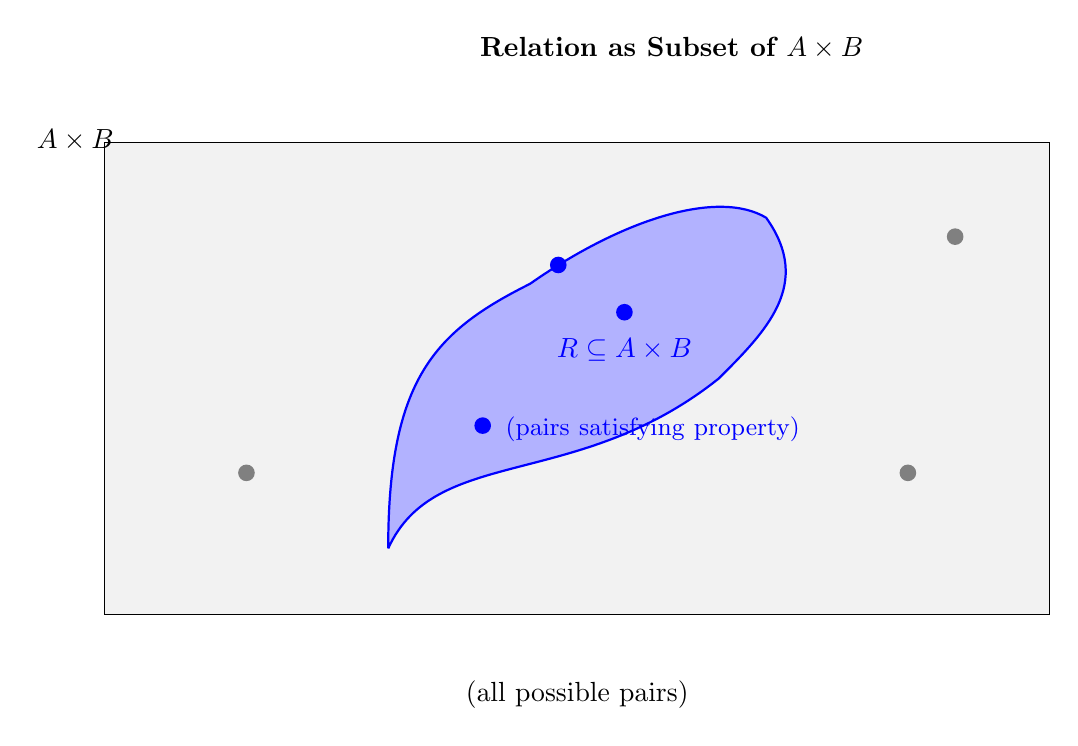
\begin{tikzpicture}[scale=1.2]
    \node at (6, 6) {\textbf{Relation as Subset of $A \times B$}};
    
    % Cartesian product
    \draw[fill=gray!10] (0,0) rectangle (10,5);
    \node[above left] at (0.2, 4.8) {$A \times B$};
    \node[below] at (5, -0.6) {(all possible pairs)};
    
    % Relation subset
    \begin{scope}
        \clip (3, 0.7) .. controls (3.5, 1.8) and (5, 1.3) .. (6.5, 2.5) 
              .. controls (7, 3) and (7.5, 3.5) .. (7, 4.2)
              .. controls (6.5, 4.5) and (5.5, 4.2) .. (4.5, 3.5)
              .. controls (3.5, 3) and (3, 2.5) .. (3, 0.7);
        \fill[blue!30] (0,0) rectangle (10,5);
    \end{scope}
    \draw[thick, blue] (3, 0.7) .. controls (3.5, 1.8) and (5, 1.3) .. (6.5, 2.5) 
                       .. controls (7, 3) and (7.5, 3.5) .. (7, 4.2)
                       .. controls (6.5, 4.5) and (5.5, 4.2) .. (4.5, 3.5)
                       .. controls (3.5, 3) and (3, 2.5) .. (3, 0.7);
    
    \node[blue] at (5.5, 2.8) {$R \subseteq A \times B$};
    \node[blue, below, text width=4cm, align=center] at (5.8, 2.2) {\small (pairs satisfying property)};
    
    % Sample points
    \fill[blue] (4, 2) circle (2.5pt);
    \fill[blue] (5.5, 3.2) circle (2.5pt);
    \fill[blue] (4.8, 3.7) circle (2.5pt);
    
    \fill[gray] (1.5, 1.5) circle (2.5pt);
    \fill[gray] (8.5, 1.5) circle (2.5pt);
    \fill[gray] (9, 4) circle (2.5pt);
\end{tikzpicture}
\end{center}

\begin{example}[Common Relations]
\begin{enumerate}
    \item \textbf{Less than on $\mathbb{N}$}:
    \[< \, := \{(m, n) \in \mathbb{N} \times \mathbb{N} : m < n\}\]
    
    \item \textbf{Divisibility}:
    \[| \, := \{(a, b) \in \mathbb{Z} \times \mathbb{Z} : a \mid b\}\]
    
    \item \textbf{Subset relation}:
    \[\subseteq := \{(A, B) \in \mathcal{P}(X) \times \mathcal{P}(X) : A \subseteq B\}\]
    
    \item \textbf{Equality}:
    \[= := \{(x, x) : x \in A\}\]
    (The diagonal of $A \times A$)
\end{enumerate}
\end{example}

\subsection{Domain, Codomain, and Image}

\begin{definition}
Let $R \subseteq A \times B$ be a relation.

\begin{itemize}
    \item The \textbf{domain} of $R$ is:
    \[\text{dom}(R) := \{a \in A : \exists b \in B, (a, b) \in R\}\]
    
    \item The \textbf{image} (or range) of $R$ is:
    \[\text{im}(R) := \{b \in B : \exists a \in A, (a, b) \in R\}\]
\end{itemize}
\end{definition}

\begin{example}
Let $A = \{1, 2, 3\}$, $B = \{a, b, c\}$, and:
\[R = \{(1, a), (1, b), (3, c)\}\]

Then:
\begin{itemize}
    \item $\text{dom}(R) = \{1, 3\}$ (element 2 doesn't relate to anything)
    \item $\text{im}(R) = \{a, b, c\}$ (all elements of $B$ are reached)
\end{itemize}
\end{example}

\section{Properties of Relations on a Single Set}

When $R \subseteq A \times A$ (relation on a set to itself), we can study structural properties.

\begin{center}
\begin{tikzpicture}[scale=1.1]
    \node at (6, 6.5) {\textbf{The Four Fundamental Properties}};
    
    % Reflexive
    \begin{scope}[shift={(0,4)}]
        \node[circle, draw, fill=blue!20] (a) at (0,0) {$a$};
        \node[circle, draw, fill=blue!20] (b) at (2,0) {$b$};
        \draw[->, thick, loop above] (a) to (a);
        \draw[->, thick, loop above] (b) to (b);
        \node[below] at (1, -0.7) {\textbf{Reflexive}: $\forall x, xRx$};
    \end{scope}
    
    % Symmetric
    \begin{scope}[shift={(5,4)}]
        \node[circle, draw, fill=green!20] (a) at (0,0) {$a$};
        \node[circle, draw, fill=green!20] (b) at (2,0) {$b$};
        \draw[->, thick, bend left] (a) to (b);
        \draw[->, thick, bend left] (b) to (a);
        \node[below] at (1, -0.7) {\textbf{Symmetric}: $xRy \implies yRx$};
    \end{scope}
    
    % Transitive
    \begin{scope}[shift={(0,0)}]
        \node[circle, draw, fill=red!20] (a) at (0,0) {$a$};
        \node[circle, draw, fill=red!20] (b) at (1.5,0) {$b$};
        \node[circle, draw, fill=red!20] (c) at (3,0) {$c$};
        \draw[->, thick] (a) to (b);
        \draw[->, thick] (b) to (c);
        \draw[->, thick, bend right=30, red] (a) to (c);
        \node[below] at (1.5, -0.7) {\textbf{Transitive}: $(xRy \land yRz) \implies xRz$};
    \end{scope}
    
    % Anti-symmetric
    \begin{scope}[shift={(5,0)}]
        \node[circle, draw, fill=yellow!40] (a) at (0,0) {$a$};
        \node[circle, draw, fill=yellow!40] (b) at (2,0) {$b$};
        \draw[->, thick] (a) to[bend left] (b);
        \draw[thick, red, cross out, line width=2pt] (1.3,0.3) -- (0.7,-0.3);
        \node[below] at (1, -0.7) {\textbf{Anti-symmetric}: $(xRy \land yRx) \implies x = y$};
    \end{scope}
\end{tikzpicture}
\end{center}

\begin{definition}[Properties of Relations]
Let $R$ be a relation on $A$ (i.e., $R \subseteq A \times A$).

\begin{enumerate}
    \item $R$ is \textbf{reflexive} if:
    \[\forall x \in A, xRx\]
    (Every element relates to itself)
    
    \item $R$ is \textbf{symmetric} if:
    \[\forall x, y \in A, (xRy \implies yRx)\]
    (Mutual relationships)
    
    \item $R$ is \textbf{transitive} if:
    \[\forall x, y, z \in A, ((xRy \land yRz) \implies xRz)\]
    (The ``chain rule'')
    
    \item $R$ is \textbf{anti-symmetric} if:
    \[\forall x, y \in A, ((xRy \land yRx) \implies x = y)\]
    (No mutual relationships except self-loops)
\end{enumerate}
\end{definition}

\begin{example}[Testing Properties]
Let $A = \{1, 2, 3, 4\}$ and $R = \{(1,1), (2,2), (3,3), (4,4), (1,2), (2,3), (1,3)\}$.

\begin{itemize}
    \item \textbf{Reflexive?} YES: $(1,1), (2,2), (3,3), (4,4) \in R$
    \item \textbf{Symmetric?} NO: $(1,2) \in R$ but $(2,1) \notin R$
    \item \textbf{Transitive?} YES: $(1,2) \in R$ and $(2,3) \in R$ and $(1,3) \in R$ $\checkmark$
    \item \textbf{Anti-symmetric?} YES: No mutual pairs except diagonal
\end{itemize}

This is a \textbf{partial order} (reflexive + anti-symmetric + transitive).
\end{example}

\begin{warning}
\textbf{Symmetric vs. Anti-symmetric}

These are NOT opposites! A relation can be:
\begin{itemize}
    \item Both (e.g., equality: $=$)
    \item Neither (e.g., ``loves'' relation among people)
    \item One but not the other
\end{itemize}

Anti-symmetric does NOT mean ``not symmetric.'' It means: if $xRy$ AND $yRx$, then $x$ must equal $y$.
\end{warning}

\section{Equivalence Relations: Generalizing Equality}

\begin{intuition}
Equality ($=$) is the most basic relation: reflexive, symmetric, transitive.

An equivalence relation generalizes equality---it groups objects that we consider ``the same'' for some purpose:
\begin{itemize}
    \item Numbers with the same remainder mod 5
    \item Geometric figures with the same shape
    \item Functions with the same limit
\end{itemize}

Equivalence relations partition a set into disjoint ``clusters'' of equivalent objects.
\end{intuition}

\begin{definition}[Equivalence Relation]
A relation $\sim$ on $A$ is an \textbf{equivalence relation} if it is:
\begin{enumerate}
    \item Reflexive: $\forall x \in A, x \sim x$
    \item Symmetric: $\forall x, y \in A, (x \sim y \implies y \sim x)$
    \item Transitive: $\forall x, y, z \in A, ((x \sim y \land y \sim z) \implies x \sim z)$
\end{enumerate}
\end{definition}

\begin{example}[Equivalence Relations]
\begin{enumerate}
    \item \textbf{Equality}: $x = y$ on any set
    
    \item \textbf{Congruence modulo $n$}: On $\mathbb{Z}$, define $a \sim b \iff n \mid (a - b)$
    
    \item \textbf{Same cardinality}: On sets, $A \sim B \iff |A| = |B|$
    
    \item \textbf{Parallel lines}: In Euclidean geometry, $\ell_1 \sim \ell_2 \iff \ell_1 \parallel \ell_2$ or $\ell_1 = \ell_2$
\end{enumerate}
\end{example}

\subsection{Equivalence Classes}

\begin{definition}[Equivalence Class]
Let $\sim$ be an equivalence relation on $A$. The \textbf{equivalence class} of $x \in A$ is:
\[[x] := \{y \in A : y \sim x\}\]

The set of all equivalence classes is called the \textbf{quotient set}:
\[A/\!\!\sim \, := \{[x] : x \in A\}\]
\end{definition}

\begin{center}
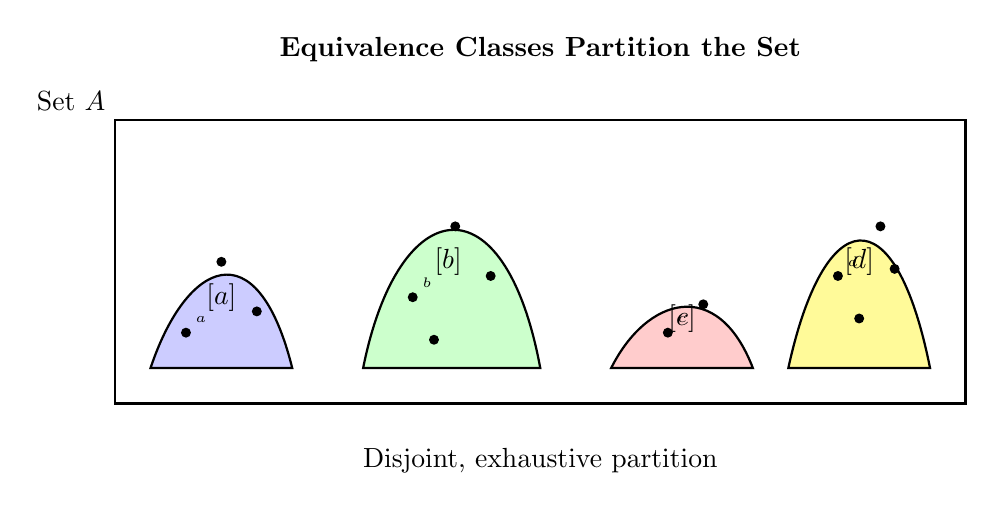
\begin{tikzpicture}[scale=0.9]
    \node at (6, 5) {\textbf{Equivalence Classes Partition the Set}};
    
    % The whole set
    \draw[thick] (0,0) rectangle (12,4);
    \node[above left] at (0,4) {Set $A$};
    
    % Class 1
    \draw[thick, fill=blue!20] (0.5,0.5) .. controls (1,2) and (2,2.5) .. (2.5,0.5) -- cycle;
    \node at (1.5,1.5) {$[a]$};
    \fill (1,1) circle (2pt) node[above right] {\tiny $a$};
    \fill (1.5,2) circle (2pt);
    \fill (2,1.3) circle (2pt);
    
    % Class 2
    \draw[thick, fill=green!20] (3.5,0.5) .. controls (4,3) and (5.5,3.2) .. (6,0.5) -- cycle;
    \node at (4.7,2) {$[b]$};
    \fill (4.2,1.5) circle (2pt) node[above right] {\tiny $b$};
    \fill (4.8,2.5) circle (2pt);
    \fill (5.3,1.8) circle (2pt);
    \fill (4.5,0.9) circle (2pt);
    
    % Class 3
    \draw[thick, fill=red!20] (7,0.5) .. controls (7.5,1.5) and (8.5,1.8) .. (9,0.5) -- cycle;
    \node at (8,1.2) {$[c]$};
    \fill (7.8,1) circle (2pt) node[above right] {\tiny $c$};
    \fill (8.3,1.4) circle (2pt);
    
    % Class 4
    \draw[thick, fill=yellow!40] (9.5,0.5) .. controls (10,2.8) and (11,3) .. (11.5,0.5) -- cycle;
    \node at (10.5,2) {$[d]$};
    \fill (10.2,1.8) circle (2pt) node[above right] {\tiny $d$};
    \fill (10.8,2.5) circle (2pt);
    \fill (10.5,1.2) circle (2pt);
    \fill (11,1.9) circle (2pt);
    
    \node[below] at (6, -0.5) {Disjoint, exhaustive partition};
\end{tikzpicture}
\end{center}

\begin{theorem}[Equivalence Classes Are Disjoint or Identical]
Let $\sim$ be an equivalence relation on $A$. For any $x, y \in A$:
\[[x] \cap [y] \neq \emptyset \implies [x] = [y]\]

Equivalently: Either $[x] = [y]$ or $[x] \cap [y] = \emptyset$.
\end{theorem}

\begin{proof}
Suppose $[x] \cap [y] \neq \emptyset$. Then there exists $z \in [x] \cap [y]$.

By definition: $z \sim x$ and $z \sim y$.

We'll show $[x] = [y]$ by proving $[x] \subseteq [y]$ and $[y] \subseteq [x]$.

($[x] \subseteq [y]$): Let $w \in [x]$. Then $w \sim x$.

We have:
\begin{itemize}
    \item $w \sim x$ (given)
    \item $x \sim z$ (by symmetry from $z \sim x$)
    \item $z \sim y$ (given)
\end{itemize}

By transitivity: $w \sim x$ and $x \sim z$ gives $w \sim z$.

Then $w \sim z$ and $z \sim y$ gives $w \sim y$.

Therefore $w \in [y]$. $\checkmark$

($[y] \subseteq [x]$): By symmetry (swapping roles of $x$ and $y$). $\checkmark$

Therefore $[x] = [y]$.
\end{proof}

\begin{theorem}[Fundamental Theorem of Equivalence Relations]
Every equivalence relation on $A$ induces a partition of $A$ (disjoint, exhaustive subsets).

Conversely, every partition of $A$ defines an equivalence relation (elements are equivalent iff they're in the same part).
\end{theorem}

\begin{proof}[Proof Sketch]
($\Rightarrow$) Given $\sim$, the equivalence classes form a partition:
\begin{itemize}
    \item \textbf{Exhaustive}: Every $x \in A$ belongs to $[x]$ (by reflexivity)
    \item \textbf{Disjoint}: By previous theorem
\end{itemize}

($\Leftarrow$) Given partition $\mathcal{P} = \{P_1, P_2, \ldots\}$, define:
\[x \sim y \iff x \text{ and } y \text{ belong to the same } P_i\]

Check this is reflexive, symmetric, transitive (exercise).
\end{proof}

\begin{example}[Integers Modulo 5]
Define $a \sim b \iff 5 \mid (a - b)$ on $\mathbb{Z}$.

This creates 5 equivalence classes:
\begin{align*}
[0] &= \{\ldots, -10, -5, 0, 5, 10, \ldots\} \\
[1] &= \{\ldots, -9, -4, 1, 6, 11, \ldots\} \\
[2] &= \{\ldots, -8, -3, 2, 7, 12, \ldots\} \\
[3] &= \{\ldots, -7, -2, 3, 8, 13, \ldots\} \\
[4] &= \{\ldots, -6, -1, 4, 9, 14, \ldots\}
\end{align*}

The quotient set $\mathbb{Z}/5\mathbb{Z} = \{[0], [1], [2], [3], [4]\}$ is the integers modulo 5.
\end{example}

\section{Order Relations: Hierarchies and Comparisons}

\begin{intuition}
While equivalence relations group things as ``same,'' order relations arrange things in a hierarchy: ``less than,'' ``subset of,'' ``precedes.''

Think of a family tree, a chain of command, or the real numbers with $\leq$.

Not all elements need to be comparable (e.g., sets under $\subseteq$: $\{1, 2\}$ and $\{3, 4\}$ are incomparable). These are \textbf{partial orders}.
\end{intuition}

\begin{definition}[Partial Order]
A relation $\preceq$ on $A$ is a \textbf{partial order} if it is:
\begin{enumerate}
    \item \textbf{Reflexive}: $\forall x \in A, x \preceq x$
    \item \textbf{Anti-symmetric}: $\forall x, y \in A, (x \preceq y \land y \preceq x) \implies x = y$
    \item \textbf{Transitive}: $\forall x, y, z \in A, ((x \preceq y \land y \preceq z) \implies x \preceq z)$
\end{enumerate}

The pair $(A, \preceq)$ is called a \textbf{partially ordered set} (poset).
\end{definition}

\begin{example}[Partial Orders]
\begin{enumerate}
    \item $(\mathbb{N}, \leq)$ --- the usual ordering
    \item $(\mathcal{P}(X), \subseteq)$ --- subset relation on power set
    \item $(X^X, \leq)$ where $f \leq g \iff \forall x, f(x) \leq g(x)$ (pointwise order on functions)
    \item Divisibility: $(a, b) \in R \iff a \mid b$ on $\mathbb{N}^+$
\end{enumerate}
\end{example}

\subsection{Hasse Diagrams}

We visualize posets using \textbf{Hasse diagrams}: elements are vertices, and $x \prec y$ (covers) is shown by $y$ above $x$ with an edge.

\begin{center}
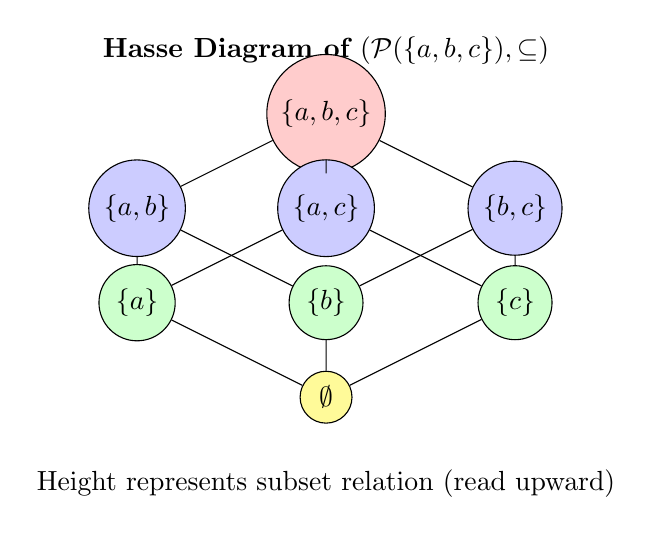
\begin{tikzpicture}[scale=0.8]
    \node at (4, 5) {\textbf{Hasse Diagram of $(\mathcal{P}(\{a,b,c\}), \subseteq)$}};
    
    % Top element
    \node[circle, draw, fill=red!20] (abc) at (4,4) {$\{a,b,c\}$};
    
    % Second level
    \node[circle, draw, fill=blue!20] (ab) at (1,2.5) {$\{a,b\}$};
    \node[circle, draw, fill=blue!20] (ac) at (4,2.5) {$\{a,c\}$};
    \node[circle, draw, fill=blue!20] (bc) at (7,2.5) {$\{b,c\}$};
    
    % Third level
    \node[circle, draw, fill=green!20] (a) at (1,1) {$\{a\}$};
    \node[circle, draw, fill=green!20] (b) at (4,1) {$\{b\}$};
    \node[circle, draw, fill=green!20] (c) at (7,1) {$\{c\}$};
    
    % Bottom
    \node[circle, draw, fill=yellow!40] (empty) at (4,-0.5) {$\emptyset$};
    
    % Edges
    \draw (empty) -- (a);
    \draw (empty) -- (b);
    \draw (empty) -- (c);
    
    \draw (a) -- (ab);
    \draw (a) -- (ac);
    \draw (b) -- (ab);
    \draw (b) -- (bc);
    \draw (c) -- (ac);
    \draw (c) -- (bc);
    
    \draw (ab) -- (abc);
    \draw (ac) -- (abc);
    \draw (bc) -- (abc);
    
    \node[below] at (4, -1.5) {Height represents subset relation (read upward)};
\end{tikzpicture}
\end{center}

\begin{definition}[Total Order]
A partial order $\preceq$ on $A$ is a \textbf{total order} (or linear order) if:
\[\forall x, y \in A, (x \preceq y \lor y \preceq x)\]

Every pair of elements is comparable.
\end{definition}

\begin{example}
\begin{itemize}
    \item $(\mathbb{R}, \leq)$ is a total order
    \item $(\mathcal{P}(\{1,2\}), \subseteq)$ is NOT: $\{1\}$ and $\{2\}$ are incomparable
\end{itemize}
\end{example}

\subsection{Special Elements in Posets}

\begin{definition}[Maximal and Minimal Elements]
Let $(A, \preceq)$ be a poset.

\begin{itemize}
    \item $m \in A$ is \textbf{maximal} if: $\forall x \in A, (m \preceq x \implies m = x)$
    
    (Nothing is strictly greater than $m$)
    
    \item $m \in A$ is \textbf{minimal} if: $\forall x \in A, (x \preceq m \implies x = m)$
    
    (Nothing is strictly less than $m$)
\end{itemize}
\end{definition}

\begin{warning}
\textbf{Maximal $\neq$ Maximum!}

In a partial order, there can be multiple maximal elements (incomparable with each other).

A \textbf{maximum} (or greatest element) $M$ satisfies: $\forall x \in A, x \preceq M$.

Example: In $(\{1,2,3,4\}, \mid)$ (divisibility), both 3 and 4 are maximal, but there's no maximum.
\end{warning}

\section{Composition of Relations}

\begin{definition}[Composition]
Let $R \subseteq A \times B$ and $S \subseteq B \times C$ be relations. The \textbf{composition} $S \circ R$ is:
\[S \circ R := \{(a, c) \in A \times C : \exists b \in B, (a, b) \in R \land (b, c) \in S\}\]
\end{definition}

\begin{center}
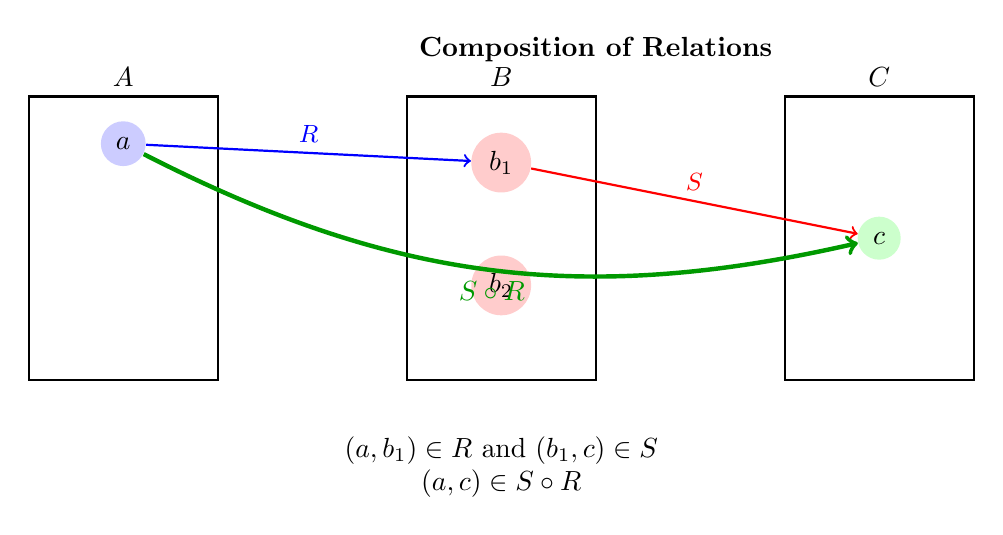
\begin{tikzpicture}[scale=1.2]
    \node at (6, 3.5) {\textbf{Composition of Relations}};
    
    % Sets
    \draw[thick] (0,0) rectangle (2,3);
    \node[above] at (1,3) {$A$};
    
    \draw[thick] (4,0) rectangle (6,3);
    \node[above] at (5,3) {$B$};
    
    \draw[thick] (8,0) rectangle (10,3);
    \node[above] at (9,3) {$C$};
    
    % Elements
    \node[circle, fill=blue!20] (a1) at (1,2.5) {$a$};
    \node[circle, fill=red!20] (b1) at (5,2.3) {$b_1$};
    \node[circle, fill=red!20] (b2) at (5,1) {$b_2$};
    \node[circle, fill=green!20] (c1) at (9,1.5) {$c$};
    
    % Relations
    \draw[->, thick, blue] (a1) -- (b1) node[midway, above] {\small $R$};
    \draw[->, thick, red] (b1) -- (c1) node[midway, above] {\small $S$};
    
    \draw[->, ultra thick, green!60!black, bend right=20] (a1) to node[below] {$S \circ R$} (c1);
    
    \node[below, align=center] at (5, -0.5) {$(a,b_1) \in R$ and $(b_1,c) \in S$ \\$\implies (a,c) \in S \circ R$};
\end{tikzpicture}
\end{center}

\begin{theorem}[Composition is Associative]
Let $R \subseteq A \times B$, $S \subseteq B \times C$, $T \subseteq C \times D$. Then:
\[T \circ (S \circ R) = (T \circ S) \circ R\]
\end{theorem}

\begin{proof}
We show both sets contain the same ordered pairs.

$(a, d) \in T \circ (S \circ R)$ 

$\iff \exists c \in C, ((a, c) \in S \circ R \land (c, d) \in T)$

$\iff \exists c \in C, ((\exists b \in B, (a, b) \in R \land (b, c) \in S) \land (c, d) \in T)$

$\iff \exists b \in B \exists c \in C, ((a, b) \in R \land (b, c) \in S \land (c, d) \in T)$

$\iff \exists b \in B, ((a, b) \in R \land (\exists c \in C, (b, c) \in S \land (c, d) \in T))$

$\iff \exists b \in B, ((a, b) \in R \land (b, d) \in T \circ S)$

$\iff (a, d) \in (T \circ S) \circ R$

Therefore the compositions are equal.
\end{proof}

\section{Looking Forward}

We have defined the general concept of a relation. Two types of relations are particularly important for the foundations of mathematics:

\begin{enumerate}
    \item \textbf{Equivalence Relations}: These allow us to construct new mathematical objects by gluing existing ones together. We will use this in the next chapter to build integers and rationals.
    \item \textbf{Functions}: These are relations that behave like ``machines''---one input, one output.
\end{enumerate}

\begin{keyidea}
\textbf{The Big Picture}:

\begin{center}
\begin{tikzpicture}[node distance=2cm]
    \node[rectangle, draw, fill=yellow!20] (sets) {Sets};
    \node[rectangle, draw, fill=red!20, right=of sets] (rel) {Relations};
    \node[rectangle, draw, fill=blue!20, right=of rel] (arith) {Arithmetic};
    \node[rectangle, draw, fill=purple!20, right=of arith] (func) {Functions};
    
    \draw[->, thick] (sets) -- (rel) node[midway, above] {\tiny subsets of $\times$};
    \draw[->, thick] (rel) -- (arith) node[midway, above] {\tiny equivalence};
    \draw[->, thick] (arith) -- (func) node[midway, above] {\tiny operations};
\end{tikzpicture}
\end{center}

Next, we will use equivalence relations to construct the number systems $\mathbb{Z}$ and $\mathbb{Q}$.
\end{keyidea}
